
\chapter{Signal Processing}
The signal processing is separated into two sections. First the code needs to be transformed into the base-band. After that a spectrum shift to a specific transmission band is realized. Afterwards the exported signal is put through an simulator which adds reflection noise. The result is than again imported and gets reverse spectrum shifted. At the end a peak detection method is used to ignore reflection peaks.
\section{Base-Band}
Before a spectrum shift is applied to the signal, the bandwidth needs to be bounded. Otherwise absolute code bits would result in theoretically infinite frequencies which are impossible to implement for transmission. A raised cosine filter is therefore applied to remove all unwanted frequencies above a certain threshold. The base-band for our application is $20kHz$. Thus, our symbol length is set to $1/{20kHz}$. A appropriate roll-off coefficient of $0.125$ is picked. The resolution of cosine needs to be high enough to include at least a couple of periods.  A whole cosine is not tangible because its periodic and therefore infinite in time.
\begin{figure}[h]
	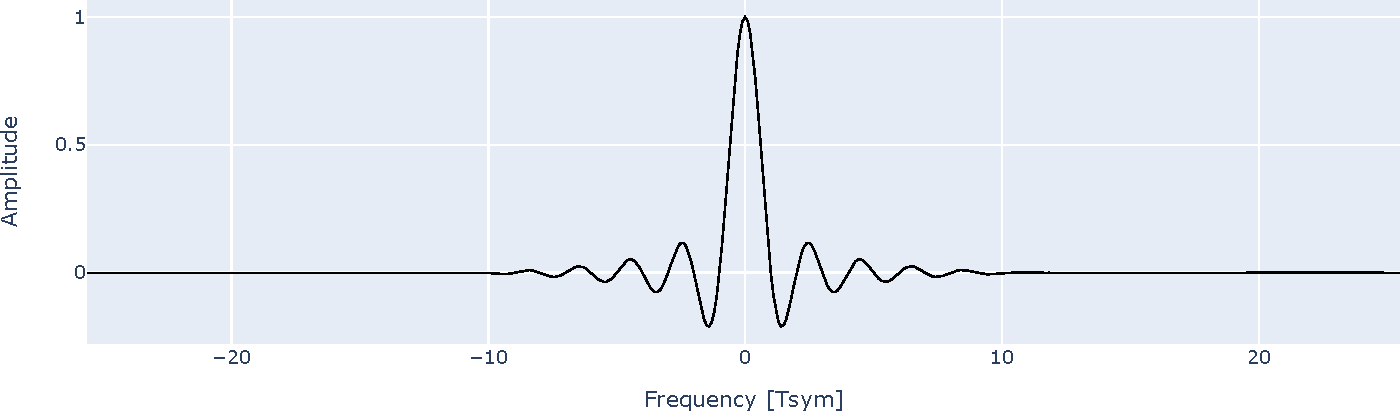
\includegraphics[width=\linewidth]{images/cosfir}
	\caption{Section of Cosine FIR with a resolution of 1024}
	\label{fig:cosfir}
\end{figure}
\section{Transmission ans Base-Band Shifting}
Now the spectrum is ready to be shifted by the given transmission frequency $f_c$. The resulting signal could hold imaginary parts, hence we only move the real part further in processing. The inverse shift works by applying the negative transmission frequency.
\begin{equation}
	x_{TB}[k]=Re\{x_{BB}[k]\cdot e^{-2\pi j f_c k}\}
	\label{eq:shift}
\end{equation}
\begin{equation}
	x_{BB}[k]=x_{TB}[k]\cdot e^{-2\pi j (-f_c) k}
	\label{eq:rshift}
\end{equation}

\section{Simulation}
The simulation consists of a watermark benchmark \cite{watermark15} and a additive GWN generated by a desired SNR between $-20dB$ and $20dB$ in steps of $5dB$. From the general equation of the Signal to Noise Ratio we derive our noise standard deviation by transforming this ratio. The white noise is added after the simulation and before receiver filtering.
\begin{equation}
	SNR=\cfrac{P_{Signal}}{P_{Noise}}=\cfrac{\mathbb{E}({Signal}^2)}{\mathbb{E}({Noise}^2)}=\cfrac{\sum {Signal}^2}{N\cdot\sigma_{Noise}^2}~~\Leftrightarrow~~\sigma_{Noise}=\sqrt{\cfrac{\sum^N {Signal}^2}{N\cdot SNR}}
\end{equation}

\begin{equation}
	SNR_{dB}=10\cdot\log_{10}\cfrac{\sum Signal^2}{\sum Noise^2}=10\cdot\log_{10}\cfrac{\sum^N_{k=1} x_{TB}^2[k]}{\sum^N_{k=1} Noise^2[k]}
\end{equation}

\begin{equation}
	Noise=\text{\textsc{Normal}}(0,1)\cdot \cfrac{\sigma_{Signal}}{SNR}
\end{equation}


\section{Low-pass Filter}

A flat magnitude is favorable because only frequencies of the base-band should be passed through. Such a filter, namely a maximally flat magnitude or Butterworth filter, approximates this goal. The roll-off decreases by increasing the order of the system.\\
The filter gets applied after shifting back to the base-band. The spectrum shift works almost the same as the first one \ref{eq:shift}, but with an sign change in the exponent. Most noise and reflections get reduced if their frequencies do not reach the base-band.
\begin{figure}[h]
	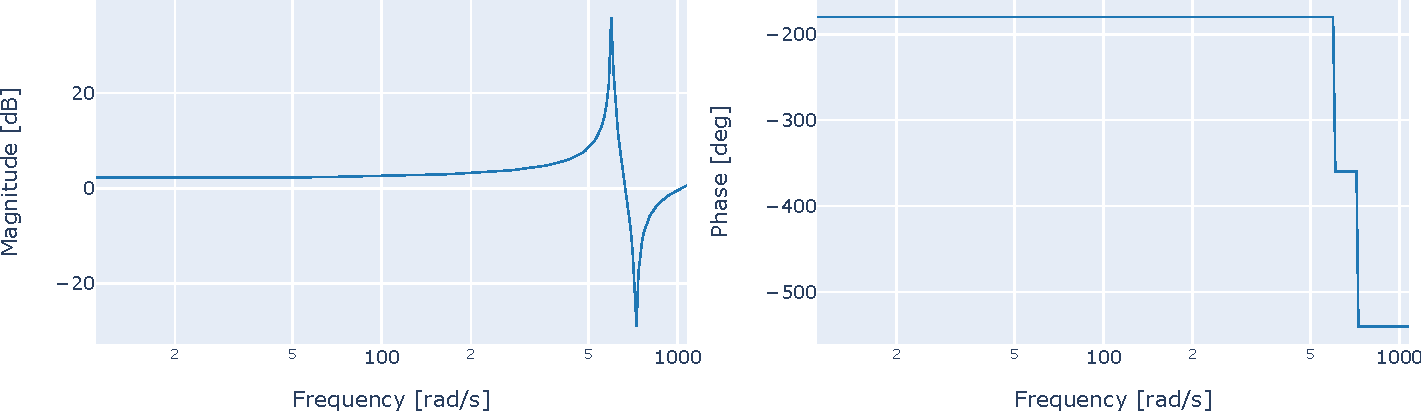
\includegraphics[width=\linewidth]{images/bode}
	
	\caption{Bode plot of 5th order Butterworth low-pass filter}
	\label{fig:bode}
\end{figure}

\section{Peak detection}
The received signal, consisting of summed delayed signals, cross-correlated by every anchor. If the signal is not reflected the peak in cross-correlation would be obvious. But because by the introduction of noise and water reflections a higher rate of similar peaks appear. To suppress these effects a CA-FAR Algorithm \cite{rohling11} is applied to only detect the first reflected peak resulting in lower false alarms of peaks. \\
CA-FAR works by using multiple values intervals. The most outer one could be described as a train bin and is used to get an estimation of the signals noise. Especially CA-FAR uses averaging to estimate the noise by measured cells. The bordering bin, defined as the guard cells, is used to reduce self-interference of the peaks. Thus, increasing window sizes $N$ resulting in better noise estimating but still limited by the sample rate \ref{eq:cft} \cite{rohling11}\cite{radarbasics}. By knowledge of measured peak widths a optimal guard interval can be figured.\\
The calculated threshold is than scaled by a formula depending on the false alarm rate. The higher the false alarm rate, the weaker high amplitude peaks gets included by the threshold \ref{eq:cff}.\\
Because Cell Averaging shows not satisfactory results in sensitive multi targets examples, the noise estimation could be enhanced by a sorting average. That principle is defined as CO-FAR \cite{rohling11}. 
\begin{center}
	\begin{tabular}{|c|c|}
		\hline
		candidate sample & $i$\\
		\hline
		guard interval (half) & $\mathcal{G}$ \\
		\hline
		train interval (half) & $\mathcal{T}$ \\
		\hline
		false alarm rate & $\eta$\\
		\hline
	\end{tabular}
	\linebreak
\end{center}

\begin{equation}
	Threshold(i)_x=
	\cfrac{\alpha}{2\mathcal{T}}
	\left[ \sum_{j=i-\left( \mathcal{G}+\mathcal{T}\right) }^{i+\left( \mathcal{G}+\mathcal{T}\right)}x(j) - \sum_{j=i-\mathcal{G}}^{i+\mathcal{G}}x(j) \right] 
	\label{eq:cft}
\end{equation}
\begin{equation}
	\text{scale factor}~~~
	\alpha=2\mathcal{T}\left( \eta^{-1/{2\mathcal{T}}}-1\right) 
	\label{eq:cff}
\end{equation}